
\documentclass{article}

\usepackage{pttyr_descriptions}


\begin{document}

\setlist{nolistsep}
\nointerlineskip
\par\noindent
\setlength{\parindent}{0pt}


\section*{Builtin Fourier Transforms}
\subsection*{\texttt{torch.stft}}
\prepostc{torch.stft(input, n\_fft, hop\_length=None, win\_length=None,
window=None, center=True, pad\_mode=`reflect', normalized=False,
onesided=True)}{
  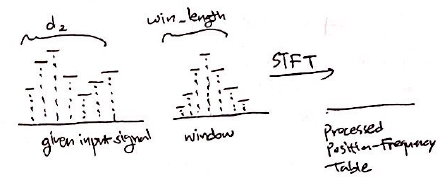
\includegraphics[height=9em]{resources/stft.png}
}{
  \begin{itemizec}
    \item $|input| = (d_1, d_2)$ or $(d_2)$\bigspace ($\mtt{rank} = 1$ or $2$)
    \item $0 < n\_fft < 2 \cdot d_2$ if $center == True$
    \item $0 < n\_fft \leq d_2$ if $center == False$
    \item $hop\_length > 0$
    \begin{itemize}
      \item if $hop\_length == None$, then let $hop\_length = \lfloor \frac{n\_fft}{4} \rfloor$.
    \end{itemize}
    \item $0 < win\_length \leq n\_fft$
    \begin{itemize}
      \item if $win\_length == None$, then let $win\_length = n\_fft$.
    \end{itemize}
    \item $window == None$ or $|window| = (win\_length)$\bigspace(rank 1)
  \end{itemizec}
}{
  \begin{itemizec}
    \item $|y| = (d_1, a, b, 2)$ or $(a, b, 2)$ ... from the proof tree
  \end{itemizec}
}{
  \begin{itemizec}
    \item 음향분석에서 자주 쓰이는 short-time Fourier transform.
    \item 마지막 텐서 부분은 real과 complex 부분을 가리키는 두 텐서.
    \texttt{real} 함수가 여기서 쓰임
  \end{itemizec}
}
\begin{align*}
  \frac
  {
    \begin{array}{l}
      \sigma \vdash E \Rar e, c \\
      \sigma \vdash window \Rar w, c_{win} \bigspace \text{if $window \neq None$, otherwise $c_{win} = \emptyset$}\\
      hop\_length = \lfloor \frac{n\_fft}{4} \rfloor \bigspace \text{if $hop\_length == None$} \\
      win\_length = n\_fft \bigspace \text{if $win\_length == None$} \\
      n = e[\op{rank}{e}] \\
      c_{dim} = \{ (window = None \lor w = (win\_length)) \land
        (0 < hop\_length) \land (0 < win\_length \leq n\_fft) \} \\
      c_{fft} = \{ (\ifs{center}{0 < n\_fft < 2 \cdot n}{0 < n\_fft < n}) \} \\
      a = \ifs{onesided}{\lfloor \frac{n\_fft}{2} \rfloor + 1}{n\_fft} \\
      b = \ifs{center}{\lfloor \frac{n}{hop\_length} \rfloor + 1}{\lfloor \frac{n - n\_fft}{hop\_length} \rfloor + 1} \\
      e' = \ifs{\op{rank}{e} == 2}{(e[1], a, b, 2)}{(a, b, 2)}
    \end{array}
  }
  {
    \sigma \vdash \op{stft}{E, n\_fft, hop\_length=None, win\_length=None, ...,
      onesided=True} \Rar e', c \cup c_{win} \cup c_{dim} \cup c_{fft}
  }
\end{align*}
Example Codes:
\begin{Verbatim}[tabsize=4,xleftmargin=2em]
a = torch.randn(5, 10000)
print(a.shape)                       # (5, 10000)
print(torch.stft(a, 4).shape)        # (5, 3, 10001, 2)
print(torch.stft(a, 200, 100).shape) # (5, 101, 101, 2)
print(torch.stft(a, 200, 100, center=False).shape) # (5, 101, 99, 2)
print(torch.stft(a, 200, 100, center=False, onesided=False).shape) # (5, 200, 99, 2)
\end{Verbatim}
  

\subsection*{\texttt{torch.rfft}}
\prepostc{torch.rfft(input, signal\_ndim, normalized=False, onesided=True)}{
  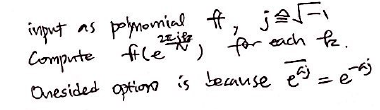
\includegraphics[height=6em]{resources/rfft.png}
}{
  \begin{itemizec}
    \item $|input| = (d_1, d_2, \dots, d_k)$
    \item $signal\_ndim \in \{1, 2, 3\}$
    \item $signal\_ndim \leq k$
  \end{itemizec}
}{
  \begin{itemizec}
    \item $|y| = (d_1, d_2, \dots, d_{k-1}, d_k', 2)$ where
    \begin{itemize}
      \item $d_k' = \ifs{onesided}{\lfloor \frac{d_k}{2} \rfloor + 1}{d_k}$
    \end{itemize}
  \end{itemizec}
}{
  \begin{itemizec}
    \item Real-to-complex Discrete Fourier Transform
    \item 마지막 텐서 부분은 real과 complex 부분을 가리키는 두 텐서.
    \texttt{real} 함수가 여기서 쓰임
  \end{itemizec}
}
\begin{align*}
  \frac
  {
    \begin{array}{l}
      \sigma \vdash E \Rar e, c \\
      k = \op{rank}{e} \\
      c_{dim} = \{ (signal\_ndim \in \{1, 2, 3\}) \land (signal\_ndim \leq k) \} \\
      f = \ifs{onesided}{\lfloor \frac{e[k]}{2} \rfloor + 1}{e[k]} \\
      e' = (e[1], e[2], \dots, e[k-1], f, 2)
    \end{array}
  }
  {
    \sigma \vdash \op{rfft}{E, signal\_ndim, normalized=False, onesided=True}
      \Rar e', c \cup c_{dim}
  }
\end{align*}


\subsection*{\texttt{torch.fft}}
\prepostc{torch.fft(input, signal\_ndim, normalized=False)}{
}{
  \begin{itemizec}
    \item $|input| = (d_1, d_2, \dots, d_k)$
    \item $d_k = 2$\bigspace (real and complex values)
    \item $signal\_ndim \in \{1, 2, 3\}$
    \item $signal\_ndim \leq k-1$
  \end{itemizec}
}{
  \begin{itemizec}
    \item $|y| = (d_1, d_2, \dots, d_{k-1}, d_k) = |input|$\bigspace (same shape)
  \end{itemizec}
}{
  \begin{itemizec}
    \item Complex-to-complex Discrete Fourier Transform
    \item 마지막 텐서 부분은 real과 complex 부분을 가리키는 두 텐서.
    \texttt{real} 함수가 여기서 쓰임
  \end{itemizec}
}
\begin{align*}
  \frac
  {
    \begin{array}{l}
      \sigma \vdash E \Rar e, c \\
      k = \op{rank}{e} \\
      c_{last} = \{ (e[k] = 2) \} \\
      c_{dim} = \{ (signal\_ndim \in \{1, 2, 3\}) \land (signal\_ndim \leq k-1) \} \\
    \end{array}
  }
  {
    \sigma \vdash \op{fft}{E, signal\_ndim, normalized=False}
      \Rar e, c \cup c_{last} \cup c_{dim}
  }
\end{align*}



\section*{Window Declarations}
\subsection*{\texttt{torch.hann\_window}}
\prepostc{torch.hann\_window(window\_length, periodic=True, dtype=None,
layout=torch.strided, device=None, requires\_grad=False)}{
}{
  \begin{itemizec}
    \item $window\_length \geq 0$
  \end{itemizec}
}{
  \begin{itemizec}
    \item $|y| = (window\_length)$
  \end{itemizec}
}{
  \begin{itemizec}
    \item $\sin^2$ 가중치의 주기성 윈도우 선언
  \end{itemizec}
}
\begin{align*}
  \frac
  {
  }
  {
    \sigma \vdash \op{hann\_window}{window\_length, ...}
      \Rar (window\_length), \{(window\_length \geq 0)\}
  }
\end{align*}


\subsection*{\texttt{torch.bartlett\_window}}
\prepostc{torch.bartlett\_window(window\_length, periodic=True, dtype=None,
layout=torch.strided, device=None, requires\_grad=False)}{
}{
  \begin{itemizec}
    \item $window\_length \geq 0$
  \end{itemizec}
}{
  \begin{itemizec}
    \item $|y| = (window\_length)$
  \end{itemizec}
}{
  \begin{itemizec}
    \item 절대값함수 가중치 윈도우 선언
  \end{itemizec}
}
\begin{align*}
  \frac
  {
  }
  {
    \sigma \vdash \op{bartlett\_window}{window\_length, ...}
      \Rar (window\_length), \{(window\_length \geq 0)\}
  }
\end{align*}


\subsection*{\texttt{torch.hamming\_window}}
\prepostc{torch.hamming\_window(window\_length, periodic=True, alpha=0.54,
beta=0.46, dtype=None,layout=torch.strided, device=None, requires\_grad=False)}{
}{
  \begin{itemizec}
    \item $window\_length \geq 0$
  \end{itemizec}
}{
  \begin{itemizec}
    \item $|y| = (window\_length)$
  \end{itemizec}
}{
  \begin{itemizec}
    \item 삼각함수 가중치의 주기성 윈도우 선언
  \end{itemizec}
}
\begin{align*}
  \frac
  {
  }
  {
    \sigma \vdash \op{hamming\_window}{window\_length, ...}
      \Rar (window\_length), \{(window\_length \geq 0)\}
  }
\end{align*}



\section*{Linear Algebra}
\subsection*{\texttt{torch.svd}}
\prepostc{torch.svd(input, some=True, compute\_uv=True, out=None)}{
  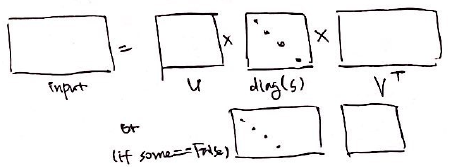
\includegraphics[height=7em]{resources/svd.png}
}{
  \begin{itemizec}
    \item $|input| = (*, m, n)$\bigspace ($\mtt{rank} \geq 2$)
  \end{itemizec}
}{
  \begin{itemizec}
    \item $|U| = (*, m, m), |S| = (*, m), |V| = ...$
    \begin{itemize}
      \item if $(compute\_uv) \land (some)$ then $|V| = (*, n, m)$\bigspace (as default)
      \item otherwise, $|V| = (*, n, n)$
    \end{itemize}
    \item $|y| = (|U|, |S|, |V|)$
  \end{itemizec}
}{
  \begin{itemizec}
    \item $(U, S, V)$ 형태의 $(Tensor, Tensor, Tensor)$ 출력 반환
    \item $input = U \x \operatorname{diag}(S) \x V^T$
    \item $out$-텐서 인자가 있는 함수
  \end{itemizec}
}
\begin{align*}
  \frac
  {
    \begin{array}{l}
      \sigma \vdash E \Rar e, c \\
      k = \op{rank}{e} \\
      u = e\indr{1}{k-2} \conc (e[k-1], e[k-1]) \\
      s = e\indr{1}{k-2} \conc (e[k-1]) \\
      v_{tail} = \ifs{(compute\_uv) \land (some)}{(n, m)}{(n, n)} \\
      v = e\indr{1}{k-2} \conc v_{tail} \\
      c_{dim} = \{ (k \geq 2) \} \\
    \end{array}
  }
  {
    \sigma \vdash \op{svd}{E, some=True, compute\_uv=True, out=None}
      \Rar (u, s, v), c \cup c_{dim}
  }
  \tag*{3-tensor tuple로 반환}
\end{align*}


\subsection*{\texttt{torch.diag}}
\prepostc{torch.diag(input, diagonal=0, out=None)}{
  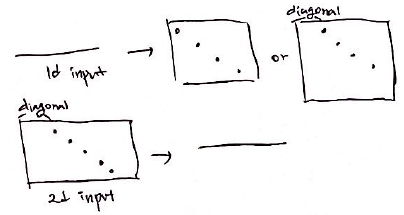
\includegraphics[height=11em]{resources/diag.png}
}{
  \begin{itemizec}
    \item $|input| = (d_1)$ or $(d_1, d_2)$. (rank 1 or 2)
    \item if $\mtt{rank} = 1$, then there is no requirement.
    \item if $\mtt{rank} = 2$, then $-d_1 \leq diagonal \leq d_2$
  \end{itemizec}
}{
  \begin{itemizec}
    \item if $\mtt{rank} = 1$, then $|y| = (d_1 + |diagonal|, d_1 + |diagonal|)$
    \item if $\mtt{rank} = 2$, then $|y| = (\min\{d_1, d_2, d_1+diagonal, d_2-diagonal\})$
  \end{itemizec}
}{
  \begin{itemizec}
    \item 1차원, 2차원 텐서 입력에 따라 역할이 달라짐
    \item $out$-텐서 인자가 있는 함수
  \end{itemizec}
}
\begin{align*}
  \frac
  {
    \begin{array}{l}
      \sigma \vdash E \Rar e, c \\
      k = \op{rank}{e} \\
      c_{dim} = \{ (k \in \{1, 2\}) \land (k = 1 \lor (-e[1] \leq diagonal \leq e[2])) \} \\
      e' = \ifs{k = 1}{(e[1] + |diagonal|, e[1] + |diagonal|)}{(\min\{e[1], e[2], e[1] + diagonal, e[2] - diagonal)\}} \\
    \end{array}
  }
  {
    \sigma \vdash \op{diag}{E, diagonal=0, out=None}
      \Rar e', c \cup c_{dim}
  }
\end{align*}


\subsection*{\texttt{torch.bilinear}, \texttt{torch.nn.functional.bilinear}}
\prepostc{torch.nn.functional.bilinear(input1, input2, weight, bias=None)}{
  %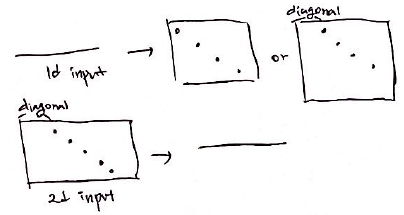
\includegraphics[height=11em]{resources/diag.png}
}{
  \begin{itemizec}
    \item $|input_1| = (d_1, d_2, \dots, d_m, h_1)$
    \item $|input_2| = (d_1, d_2, \dots, d_m, h_2)$
    \begin{itemize}
      \item Same ranks with $\mtt{rank} \geq 1$ and
      \item for all $i \in \{1, 2, \dots, m\}$, $|input_1|[i] = |input_2|[i]$
    \end{itemize}
    \item $|weight| = (s, h_1, h_2)$
    \item $bias$ is $None$ or $|bias| = (s)$
  \end{itemizec}
}{
  \begin{itemizec}
    \item $|y| = (d_1, d_2, \dots, d_m, s)$
  \end{itemizec}
}{
  \begin{itemizec}
    \item 특이사항으로 \texttt{torch.nn.functional.bilinear}에서는
    \texttt{bias}의 기본값이 $None$으로 설정되어있지만,
    \texttt{torch.bilinear}에서는 그렇지 않아서 무조건 값을 넣어줘야합니다.
  \end{itemizec}
}
\begin{align*}
  \frac
  {
    \begin{array}{l}
      \sigma \vdash E_1 \Rar e_1, c_1 \\
      \sigma \vdash E_2 \Rar e_2, c_2 \\
      \sigma \vdash W \Rar w, c_w \\
      \sigma \vdash B \Rar b, c_b \bigspace \text{if $B$ is not $None$, otherwise $c_b = \emptyset$} \\
      c_{dim} = \{ (\op{rank}{e_1} = \op{rank}{e_2}) \land (\op{rank}{e_1} \geq 1)
        \land (\op{rank}{w} = 3) \} \\
      k = \op{rank}{e_1} \\
      c_{prefix} = \{ (\forall i \in \{1, 2, \dots, k-1\}, e_1[i] = e_2[i]) \} \\
      c_{suffix} = \{ (e_1[k] = w[2]) \land (e_2[k] = w[3]) \land (B = None \lor b = (w[1])) \} \\
      e' = e_1\indr{1}{k-1} \conc (w[1])
    \end{array}
  }
  {
    \sigma \vdash \op{bilinear}{E_1, E_2, W, B=None}
      \Rar e', c \cup c_{dim} \cup c_{prefix} \cup c_{suffix}
  }
\end{align*}

\end{document}
